\section{Monte Carlo Methods}

Monte Carlo methods in RL are a class of algorithms that rely on \hyperref[sec:repeated-random-sampling]{\emph{repeated random sampling}} and average the sample returns. They are used to estimate the value functions and discover optimal policies. Monte Carlo methods are used when the agent's environment is modeled as a Markov Decision Process (MDP), but the agent does not have complete knowledge of the environment. In particular, it does not know the transition probabilities and rewards for each state. Instead, it learns from experience by sampling episodes of experience from the environment. The \emph{experience}, sequences of states, actions, and rewards, are the only information required to apply Monte Carlo methods. We define Monte Carlo methods only for episodic tasks. That is, the experience is divided into episodes and all episodes will eventually terminate.

To conclude, the key characteristics of Monte Carlo methods are:

\begin{itemize}
    \item \textbf{Model-free}: Monte Carlo methods do not require a model of the environment's dynamics.
    \item \textbf{Episodic-based}: Monte Carlo methods learn from complete episodes. They do not \hyperref[sec:bootstrapping]{bootstrap}.
    \item \textbf{Sampled returns}: Monte Carlo methods use the \emph{empirical mean return} rather than the \emph{expected return} to estimate the value functions.
\end{itemize}

\subsection{Monte Carlo Prediction}

First, we would like to learn the state-value function for a given policy with Monte Carlo methods. The value of a certain state, the expected return, is the expected cumulative future discounted reward starting from that state. To estimate from experience, we can simply average the returns observed after visits to that state. \emph{As more returns are observed, by the law of large numbers, the average should converge to the expected value.} This idea is the basis of Monte Carlo prediction.

\begin{algorithm}
    \caption{\hyperref[sec:fv-ev]{First-visit} MC prediction, for estimating $V \approx v_\pi$}\label{alg:FV-MC-V}
    \begin{algorithmic}
        \State Input: a policy $\pi$ to be evaluated
        \State Initialize:
        \State \hspace{\algorithmicindent} $V(s) \in \mathbb{R}$, arbitrarily, for all $s \in \mathcal{S}$
        \State \hspace{\algorithmicindent} $Returns(s) \leftarrow$ an empty list, for all $s \in \mathcal{S}$
        \Loop{ for each episode}
        \State Generate an episode following $\pi$: $S_0, A_0, R_1, S_1, A_1, R_2, \dots, S_{T-1}, A_{T-1}, R_T$
        \State $G \leftarrow 0$
        \For{$t = T-1, T-2, \dots, 0$}
        \State $G \leftarrow \gamma G + R_{t+1}$
        \If{$S_t$ not in $S_0, S_1, \dots, S_{t-1}$}
        \State Append $G$ to $Returns(S_t)$
        \State $V(S_t) \leftarrow \text{average}(Returns(S_t))$
        \EndIf
        \EndFor
        \EndLoop
    \end{algorithmic}
\end{algorithm}

Detailed explanation of Algorithm~\ref{alg:FV-MC-V}:

Initialize:
\begin{itemize}
    \item $V(s)$: value function in state $s$.
    \item $Returns(s)$: total rewards in state $s$.
\end{itemize}

Loop for each episode:
\begin{itemize}
    \item Generate an episode: how we use the policy.
    \item $G$:  the total return from the current state to the end of the episode.
    \item if $S_t$ not in $S_0, S_1, \dots, S_{t-1}$: check if it is the first visit to state $S_t$. This clause will ensure that we only count the first visit to state $S_t$.
    \item $V(S_t) \leftarrow \text{average}(Returns(S_t))$: the average here is the key idea of MC methods, the utilization of the law of large numbers.
\end{itemize}

Now let's talk about why we did a backward loop in each episode to update the total return. The reason is very intuitive since the return $G_t$ from a state $S_t$ is the total discounted reward received from time $t$ \emph{onwards} until the end of the episode:

\begin{align*}
    G_t &= R_{t+1} + \gamma R_{t+2} + \gamma ^2 R_{t+3} + ... + \gamma ^{T-t-1} R_{T} \\
    &= R_{t+1} + \gamma G_{t+1}
\end{align*}

Since $R_T$ is the immediate reward provided by the terminal state, $G_T$ is always 0. In this case, $G_{T-1} = R_T + \gamma G_T = R_T$ and it's really easy to start at this point.

\begin{align*}
    G_{T-1} &= R_T + \gamma G_T = R_T\\
    G_{T-2} &= R_{T-1} + \gamma G_{T-1} = R_{T-1} + \gamma R_T\\
    G_{T-3} &= R_{T-2} + \gamma G_{T-2} = R_{T-2} + \gamma R_{T-1} + \gamma ^2 R_T\\
    &\vdots\\
    G_1 &= R_2 + \gamma G_2 = R_2 + \gamma R_3 + \gamma ^2 R_4 + ... + \gamma ^{T-2} R_T\\
    G_0 &= R_1 + \gamma G_1 = R_1 + \gamma R_2 + \gamma ^2 R_3 + ... + \gamma ^{T-1} R_T
\end{align*}

\begin{minipage}[c]{0.9\textwidth}
    Why can we do the calculation like this? Because the Monte Carlo diagram goes all the way to the end of the episode and there is no diversion. As the backup diagram shows, the white circles are states, the black dots are actions and the gray square is the terminal state.

    \vspace{1em}
    Another important fact about Monte Carlo methods is that the estimates for each state are independent.
    
    \vspace{1em}
    Above all, I think that's why we chose to start at the end of the episode to update the total return.
\end{minipage}
\hfill
\begin{minipage}[c]{0.1\textwidth}
    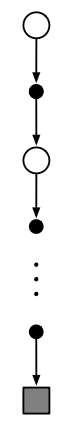
\includegraphics[height = 3\textwidth]{Figures/MC_diagram.png}
\end{minipage}

\subsection{Monte Carlo Control}

\begin{minipage}[c]{0.8\textwidth}
    The Monte Carlo estimation can be used in approximate optimal policies and we call it Monte Carlo control. As we discussed in the DP chapter, the idea of generalized policy iteration (GPI) is combined with policy evaluation and policy improvement. In Monte Carlo control, the value function $Q$ is repeatedly altered to approximate the value function for the current policy $q_\pi$ (policy evaluation). The policy $\pi$ is repeatedly improved by making \emph{greedy} actions on the current value function (policy improvement). Those two processes work together to produce both optimal value function and policy.
\end{minipage}
\hfill
\begin{minipage}[c]{0.2\textwidth}
    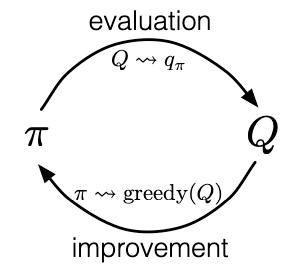
\includegraphics[height = 1.3\textwidth]{Figures/MC_GPI.png}
\end{minipage}

Policy prediction is done as presented previously. Assume that we observed an infinite number of episodes and go with exploring starts. Under these assumptions, the Monte Carlo methods will compute each expected reward, $q_{\pi_k}$, exactly for $\pi_k$, $k$ is the step number. These assumptions will also ensure that the Monte Carlo methods will converge. \emph{To obtain practical algorithms, we need to remove these assumptions.} As for how to remove exploring starts, we will discuss it later. For how to remove the infinite number of episodes, just think about that we move the value function towards $q_{\pi_k}$, but we do not expect to actually get close except over \emph{many steps}.

Policy improvement is done by making the policy greedy with respect to the current value function. That is, for each state $s$, we set $\pi(s) = \arg\max_a q(s,a)$.

\subsection{Monte Carlo Control with \texorpdfstring{\hyperref[sec:exploring-start]{Exploring Starts}}{Exploring Starts}}

\begin{algorithm}
    \caption{Monte Carlo Exploring Starts, for estimating $\pi \approx \pi_*$}\label{alg:MC_ES}
    \begin{algorithmic}
        \State Initialize:
        \State \hspace{\algorithmicindent} $\pi(s) \in \mathcal{A}(s)$, arbitrarily, for all $s \in \mathcal{S}$
        \State \hspace{\algorithmicindent} $Q(s,a) \in \mathbb{R}$, arbitrarily, for all $s \in \mathcal{S}, a \in \mathcal{A}(s)$
        \State \hspace{\algorithmicindent} $Returns(s,a) \leftarrow$ an empty list, for all $s \in \mathcal{S}, a \in \mathcal{A}(s)$
        \Loop{ for each episode}
        \State Choose $S_0 \in \mathcal{S}$ and $A_0 \in \mathcal{A}(S_0)$ such that all pairs have probability $> 0$
        \State Generate an episode from $S_0$, $A_0$ following $\pi$: $S_0$, $A_0$, $R_1$, $S_1$, $A_1$, $R_2$, $\dots$, $S_{T-1}, A_{T-1}, R_T$
        \State $G \leftarrow 0$
        \For{$t = T-1, T-2, \dots, 0$}
        \State $G \leftarrow \gamma G + R_{t+1}$
        \If{$(S_t, A_t)$ not in $S_0, A_0, S_1, A_1, \dots, S_{t-1}, A_{t-1}$}
        \State Append $G$ to $Returns(S_t, A_t)$
        \State $Q(S_t, A_t) \leftarrow \text{average}(Returns(S_t, A_t))$
        \State $\pi(S_t) \leftarrow \arg\max_a Q(S_t, a)$
        \EndIf
        \EndFor
        \EndLoop
    \end{algorithmic}
\end{algorithm}

Detailed explanation of Algorithm~\ref{alg:MC_ES}:

\begin{itemize}
    \item Q(s,a): value function in state $s$ when taking action $a$. Here we need to maintain the state-action pair so the annotation is $Q(s,a)$ rather than $V(s)$.
    \item Returns(s,a): total rewards in state $s$ when taking action $a$. Here we also need to maintain the state-action pair.
    \item $\pi(S_t) \leftarrow \arg\max_a Q(S_t, a)$: the greedy policy for a certain state $s$ at time $t$ is to choose the action $a$ that maximizes the value function $Q(s,a)$.
\end{itemize}

\subsection{On-policy and Off-policy}

\subsubsection{Behavior policy and Target policy}

\begin{itemize}
    \item \textbf{Behavior policy}: The agent follows to explore and interact with the environment during the learning process. It dictates the agent's actions based on its current state. The primary role of the behavior policy is to ensure sufficient \emph{exploration} of the environment.
    \item \textbf{Target policy}: The agent is actually trying to optimize or learn. This is the policy that the agent aspires to follow once it has learned enough about the environment. The target policy is focused on \emph{exploitation}, meaning it aims to maximize the expected reward or value based on the current knowledge of the environment.
\end{itemize}

\subsubsection{On-policy and Off-policy}

\begin{itemize}
    \item \textbf{On-policy}: The policy that the agent is learning is the same as the policy it is using to make decisions during its interaction with the environment.
    \item \textbf{Off-policy}: The policy that the agent is learning is different from the policy it is using to interact with the environment.
\end{itemize}

From my perspective, on-policy methods could be considered a special case of off-policy methods in which the target policy and behavior policy are the same.

\subsection{On-policy Monte Carlo Control}

What about avoiding the assumption of exploring starts? Let's consider on-policy Monte Carlo Control first.

In on-policy control problems, the policy is generally \emph{soft}, meaning that $\pi(a|s) > 0$ for all $s \in \mathcal{S}$ and $a \in \mathcal{A}(s)$, but gradually shifted closer and closer to a deterministic optimal policy.

We have talked about $\epsilon$-greedy policy, which adopts a very small probability, $\epsilon$ for exploration and $1-\epsilon$ for exploitation. Basically, $\epsilon$-greedy policy is a subset of $\epsilon$-soft policy. As for $\epsilon$-soft policy, the agent ensures that the probability of every action being selected in every state is at least 
$\epsilon$, but it's not constrained to be exactly $\epsilon$. When using $\epsilon$-soft policy, the policy is soft with respect to the condition that all actions have some probability greater than zero of being chosen. Here we can just use a simple $\epsilon$-soft policy. All non-greedy actions are given the minimal probability of selection, $\frac{\epsilon}{|\mathcal{A}(s)|}$ and for greedy actions, the probability of selection is $1-\epsilon + \frac{\epsilon}{|\mathcal{A}(s)|}$.

Now with first-visit methods, we can compose the on-policy first-visit Monte Carlo Control Algorithm~\ref{alg:MC_on_policy} for $\epsilon$-soft policies.

\begin{algorithm}
    \caption{On-policy first-visit MC control (for $\epsilon$-soft policies), estimating $\pi \approx \pi_*$}\label{alg:MC_on_policy}
    \begin{algorithmic}
        \State Initialize:
        \State \hspace{\algorithmicindent} $\pi(s) \in \mathcal{A}(s)$, arbitrarily, for all $s \in \mathcal{S}$
        \State \hspace{\algorithmicindent} $Q(s,a) \in \mathbb{R}$, arbitrarily, for all $s \in \mathcal{S}, a \in \mathcal{A}(s)$
        \State \hspace{\algorithmicindent} $Returns(s,a) \leftarrow$ an empty list, for all $s \in \mathcal{S}, a \in \mathcal{A}(s)$
        \Loop{ for each episode}
        \State Generate an episode following $\pi$: $S_0, A_0, R_1, S_1, A_1, R_2, \dots, S_{T-1}, A_{T-1}, R_T$
        \State $G \leftarrow 0$
        \For{$t = T-1, T-2, \dots, 0$}
        \State $G \leftarrow \gamma G + R_{t+1}$
        \If{$(S_t, A_t)$ not in $S_0, A_0, S_1, A_1, \dots, S_{t-1}, A_{t-1}$}
        \State Append $G$ to $Returns(S_t, A_t)$
        \State $Q(S_t, A_t) \leftarrow \text{average}(Returns(S_t, A_t))$
        \State $A^* \leftarrow \arg\max_a Q(S_t, a)$
        \For{$a \in \mathcal{A}(S_t)$}
        \If{$a = A^*$}
        \State $\pi(a|S_t) \leftarrow 1 - \epsilon + \frac{\epsilon}{|\mathcal{A}(S_t)|}$
        \Else
        \State $\pi(a|S_t) \leftarrow \frac{\epsilon}{|\mathcal{A}(S_t)|}$
        \EndIf
        \EndFor
        \EndIf
        \EndFor
        \EndLoop
    \end{algorithmic}
\end{algorithm}

\subsection{Off-policy Monte Carlo Control}

In off-policy methods, the behavior policy and the target policy will be different. An advantage of this separation is that the target policy may be deterministic, while the behavior policy can continue to sample all possible actions. We can compose an algorithm for off-policy Monte Carlo control with importance sampling.

Here are some detailed explanation of Algorithm~\ref{alg:MC_off_policy}:

In the initialization part, $\pi(s) \leftarrow \arg\max_a Q(s,a)$ means the action that, according to the current estimates of the action-value function $Q(s,a)$, is the best action to take in state $s$. It means that the algorithm starts by assuming that the best action to take in any state is the one that currently looks to be the best.

The phrase ``with ties broken consistently'' means that if there are multiple actions with the same value, there should be a consistent rule for which action is chosen as the best. This could be as simple as always choosing the first action in the list, or something more complex, but it should be applied consistently throughout the learning process.

\begin{algorithm}
    \caption{Off-policy MC control, for estimating $\pi \approx \pi_*$}\label{alg:MC_off_policy}
    \begin{algorithmic}
        \State Initialize:
        \State \hspace{\algorithmicindent} $Q(s,a) \in \mathbb{R}$, arbitrarily, for all $s \in \mathcal{S}, a \in \mathcal{A}(s)$
        \State \hspace{\algorithmicindent} $C(s,a) \leftarrow 0$, for all $s \in \mathcal{S}, a \in \mathcal{A}(s)$
        \State \hspace{\algorithmicindent} $\pi(s) \leftarrow \arg\max_a Q(s,a)$, for all $s \in \mathcal{S}$ (with ties broken consistently)
        \Loop{ for each episode}
        \State $b \leftarrow$ any soft policy
        \State Generate an episode following $b$: $S_0, A_0, R_1, S_1, A_1, R_2, \dots, S_{T-1}, A_{T-1}, R_T$
        \State $G \leftarrow 0$
        \State $W \leftarrow 1$
        \For{$t = T-1, T-2, \dots, 0$}
        \State $G \leftarrow \gamma G + R_{t+1}$
        \State $C(S_t, A_t) \leftarrow C(S_t, A_t) + W$
        \State $Q(S_t, A_t) \leftarrow Q(S_t, A_t) + \frac{W}{C(S_t, A_t)} \left[ G - Q(S_t, A_t) \right]$
        \State $\pi(S_t) \leftarrow \arg\max_a Q(S_t, a)$
        \If{$A_t \neq \arg\max_a Q(S_t, a)$}
        \State Exit loop
        \EndIf
        \State $W \leftarrow W \frac{1}{b(A_t|S_t)}$
        \EndFor
        \EndLoop
    \end{algorithmic}
\end{algorithm}

\subsection{Compare with Dynamic Programming}

Let's recall the Bellman equation for the optimal state-value function:

\[v_*(s) = \max_a\sum_{s', r} p(s',r|s,a) \left[ r + \gamma v_*(s')\right]\]

In Dynamic Programming, we need to know the \emph{transition matrix} as well as the \emph{reward system}, but it is not always the realistic condition. In reality, we may not know $p(s',r|s,a)$. In this case, we cannot compute $V(s)$. By adopting Monte Carlo methods, we play enough number of episodes of the game and extract the information needed.

In DP, we didn't play the game because we already knew the dynamics of the game, which is at each state we knew what are the probabilities of going to another state when we took certain actions, and we knew what the reward was going to be. In Monte Carlo methods, we don't know those data unless we play the game. That's the key difference between DP and MC methods.

\subsection*{Appendix}

\subsubsection*{Repeated random sampling}\label{sec:repeated-random-sampling}

Repeated random sampling is a statistical technique where subsets, or samples, are taken from a larger population or dataset while each sample is selected randomly. The idea behind repeated random sampling is to obtain a representative subset of the larger population, which can be analyzed to infer the properties of the entire population. Each sample should be selected using a process that gives every possible sample an \emph{equal} chance of being chosen.

Here are some sampling techniques that may be employed:

\begin{itemize}
    \item \textbf{Simple random sampling}: Every member of the population has an equal chance of being included in the sample.
    \item \textbf{Stratified sampling}: The population is divided into mutually exclusive groups, called strata, and random samples are taken from each stratum.
    \item \textbf{Cluster sampling}: The population is divided into mutually exclusive groups, called clusters, and then all members of the clusters are included in the sample.
\end{itemize}

\subsubsection*{Bootstrapping in Monte Carlo methods}\label{sec:bootstrapping}

Bootstrapping refers to the process of updating estimates based on other current estimates rather than waiting until the final outcome is known.

Monte Carlo methods \emph{do not} bootstrap. Because they update the value function only at the end of an episode, based on the entire sequence of observed rewards from the episode. They use the total accumulated reward from the current state until the end of the episode to update the value function. In this case, the value function for a certain state is updated based on the \emph{actual rewards} rather than the \emph{expected rewards}.

\subsubsection*{First-visit and every-visit Monte Carlo methods}\label{sec:fv-ev}

Each occurrence of state $s$ in an episode is called a \emph{visit} to $s$.
\begin{itemize}
    \item \textbf{First-visit}: The first time-step $t$ that state $s$ is visited in an episode.
    \item \textbf{Every-visit}: Every time-step $t$ that state $s$ is visited in an episode.
\end{itemize}

First-visit Monte Carlo methods estimate the value of a state as the average of the returns following first visits to that state. Every-visit Monte Carlo methods estimate the value of a state as the average of the returns following all visits to that state. The two methods converge to the true value function as the number of visits to each state goes to infinity. Notice that there is no guarantee to pass by all states.

It seems that Every-visit Monte Carlo methods can make better use of data. In this case, why do we still need First-visit ones? As for First-visit, it is simpler and easier to implement. Besides, it has less bias, since it only considers the first visit in an episode, it reduces the bias that might come from the peculiarities of a specific episode. As a result, it is particularly useful when the environment has low stochasticity or when the policy does not significantly change over time. In comparison, every-visit method makes use of all the data available in an episode, which can be particularly beneficial in environments with high variance or noise. It can converge faster to the true value function in certain environments, especially when the number of episodes is limited. So, it is effective in highly stochastic environments or when the policy changes frequently, as it can capture more varied experiences.

To summarize, how should one choose which method to use? In general, the choice depends on the specific characteristics of the environment and the task, as well as the consideration of efficiency. Furthermore, every-visit methods may be more aligned with exploration strategies, while first-visit methods might emphasize exploiting known, effective strategies.

In this section, we will solely focus on first-visit Monte Carlo methods.

\subsubsection*{Exploring start}\label{sec:exploring-start}

As we mentioned in the last section, Monte Carlo prediction is adopted to estimate the value function $q_\pi(s,a)$ when starting in state $s$, taking action $a$ and following policy $\pi$.

Regardless of whether we opt for the first-visit or every-visit Monte Carlo method, the only complication is that some state-action pairs may never be visited. If the $\pi$ is stochastic, then $\pi(a|s)$ represents the \emph{probability} that $a$ is chosen while in state $s$. If the policy $\pi$ is deterministic, for every state $s$, the $\pi$ will choose one specific action $a$ to take which means $\pi(s)=a$. In this case, except for one action, all other actions will have no returns to average and the MC estimates of these actions will not improve with experience. This is the problem of how to maintain exploration.

To guarantee that all state-action pairs are visited, we assume that the agent starts in a state-action pair and every pair has a nonzero probability of being selected as the start. This method is called \emph{exploring start}.

\subsubsection*{Importance sampling}\label{sec:importance-sampling}

Why do we need importance sampling? When doing off-policy prediction, the agent seeks to learn the optimal behavior, but they need to behave non-optimal to explore. In this case, the problem is how can the agent learn about the optimal policy while behaving according to an exploratory policy. The on-policy is a compromise that utilizes a near-optimal policy to do exploitation while keeping exploration. For off-policy, we utilize two policies.

